\documentclass[11pt,a4paper]{report}
\usepackage{graphicx}
\usepackage{float}
\usepackage{multicol}
\usepackage[dvipsnames]{xcolor}

\textwidth=450pt
\oddsidemargin=0pt
\begin{document}

\title{Title}

\section*{Introduction}
The project I developed follows the call to the Brain Challenge. An initiative of \dots \dots.
An entire set of MRI images of the brains of different people is provided along with other personal data like age, gender and site of collection of the images. The images were previously processed through an algorithm of features extraction that collected a series of about 1000 properties of each one of the 2000 patients. A database was made of all this information.

My contribution to this work is a statistical analysis of the relationship between the features of the images and the age of the people under survey. The method I devised is based on a significant reduction in the dimensionality of the features space and a following regression in order to detect a predictive model for the age of the people starting from those images. A possible added value to this work is the possibility to infer a biological interpretation of the most influential features for the age prediction purpose.

In particular I managed the dimensionality reduction exploiting the ridge penalized regression model on the standardized dataset and extracted the 50 most influential features. I further conducted a single vector regression on that reduced space to make a prediction of the age of the samples that resulted in a good predictor with a $R^{2}$ score about 0.7?. In order to show the quality of the fitting I made use of a gaussian process regressor that provide a good representation of the confidence interval of the model.


\section*{Brain Challenge}
Don't now anything about the challenge, waiting for further information.

My work started with a dataframe with about 1000 features collected on almost 2000 samples  (\texttt{n\_features} = 959 and \texttt{n\_samples} = 2364). Five columns of the dataset provide personal information as age, gender, site of medical analysis and the subject ID. The other 954 quantities contain the values of all the computed features as float number.

[Here I should add a couple of graphs of abundance of ages in respect to gender and in respect to site of analysis]


% This project aim to analyze the relationship between a bunch of features computed on several NRM images of the brain of different patients and the age of those patients. The final purpose of this analysis is to attempt to detect those images' features that are better able to predict the patient's age and try to extract the biological meaning from this information. Some simple regression methods performed well on the entire dataset and received a $R^{2} = 0.792$, but the aim is to find a restricted set of features with a not so lower score. I've found that a restricted set of 50 features was able to predict the age of the sample with a $R^{2}$ equal to 0.73 [This result should be verified in the last run]. This is a good result considering that the dimensionality has been reduced about 200 times.


\subsection*{Methods}


The raw images database had already been pre-processed when it was given to me. Therefore my work started with a dataframe with about 1000 features collected on almost 2000 samples (\texttt{n\_features} = 954 and \texttt{n\_samples} = 2364). I've written all the necessaries scripts using Python and more precisely I've exploited a lot of methods form the package \texttt{scikitlearn}. Before the analysis I split the dataset into two parts: 90\% for the training and the remaining 10\% for the testing part.

\subsection*{Dimensionality Reduction}
The reduction in the number of features is one of the key point of this analysis. I wanted to conserve the meaning of each features in the reduced space so I avoided the use of any dimensionality reduction method that worked with a combination of features as PCA. Hence I used different combinations of scaler method, to standardize the data, and penalized linear model like ridge, Lasso and the elastic net model. The coefficients of these regressions have been used as scores in the determination of which were the most predictive features.

More precisely, I used three different method to standardize the data: the \texttt{MinMaxScaler}, the \texttt{StandardScaler} and the \texttt{RobustScaler}. The \texttt{MinMaxScaler} scales the each feature individually to the range $\lbrack 0,1 \rbrack$, and it's the one that received the best scores among the three. The \texttt{StandardScaler} modify each single column simply setting the mean to 0 and the standard deviation to 1. The \texttt{RobustScaler} instead, manage every feature giving less importance to outliers.

Those scaling methods were combined with three penalized regression methods: the \texttt{LassoCV}, the \texttt{RidgeCV}, and the \texttt{ElasticNetCV}.All these three supervised methods are linear in the coefficients. What you obtain after such a regression is the array of values that express the linear combination of features that better predict the age of the samples. Every one of these methods find the best hyper-parameters for the regression and perform automatically a cross validation on their results.  The Lasso regression exerts a penalization on the L1-norm of the coefficients vector, the ridge regression instead is based on the L2-norm of the vector, while the elastic net method performs a sort of mixture of the two methods.

The total number of combinations among these elements is 9. So I processed the data with each one of them and obtained nine arrays of coefficients. Then I was able to sort the absolute values of those coefficients in order to find the most important ones for every combination. These results are shown in Figure \ref{fig:NineCoefPlot}. The 9 sets of values reported in \ref{fig:NineCoefPlot} were used to find those values to use as thresholds in selecting the most important features.

\begin{figure}[H]
  \begin{center}
  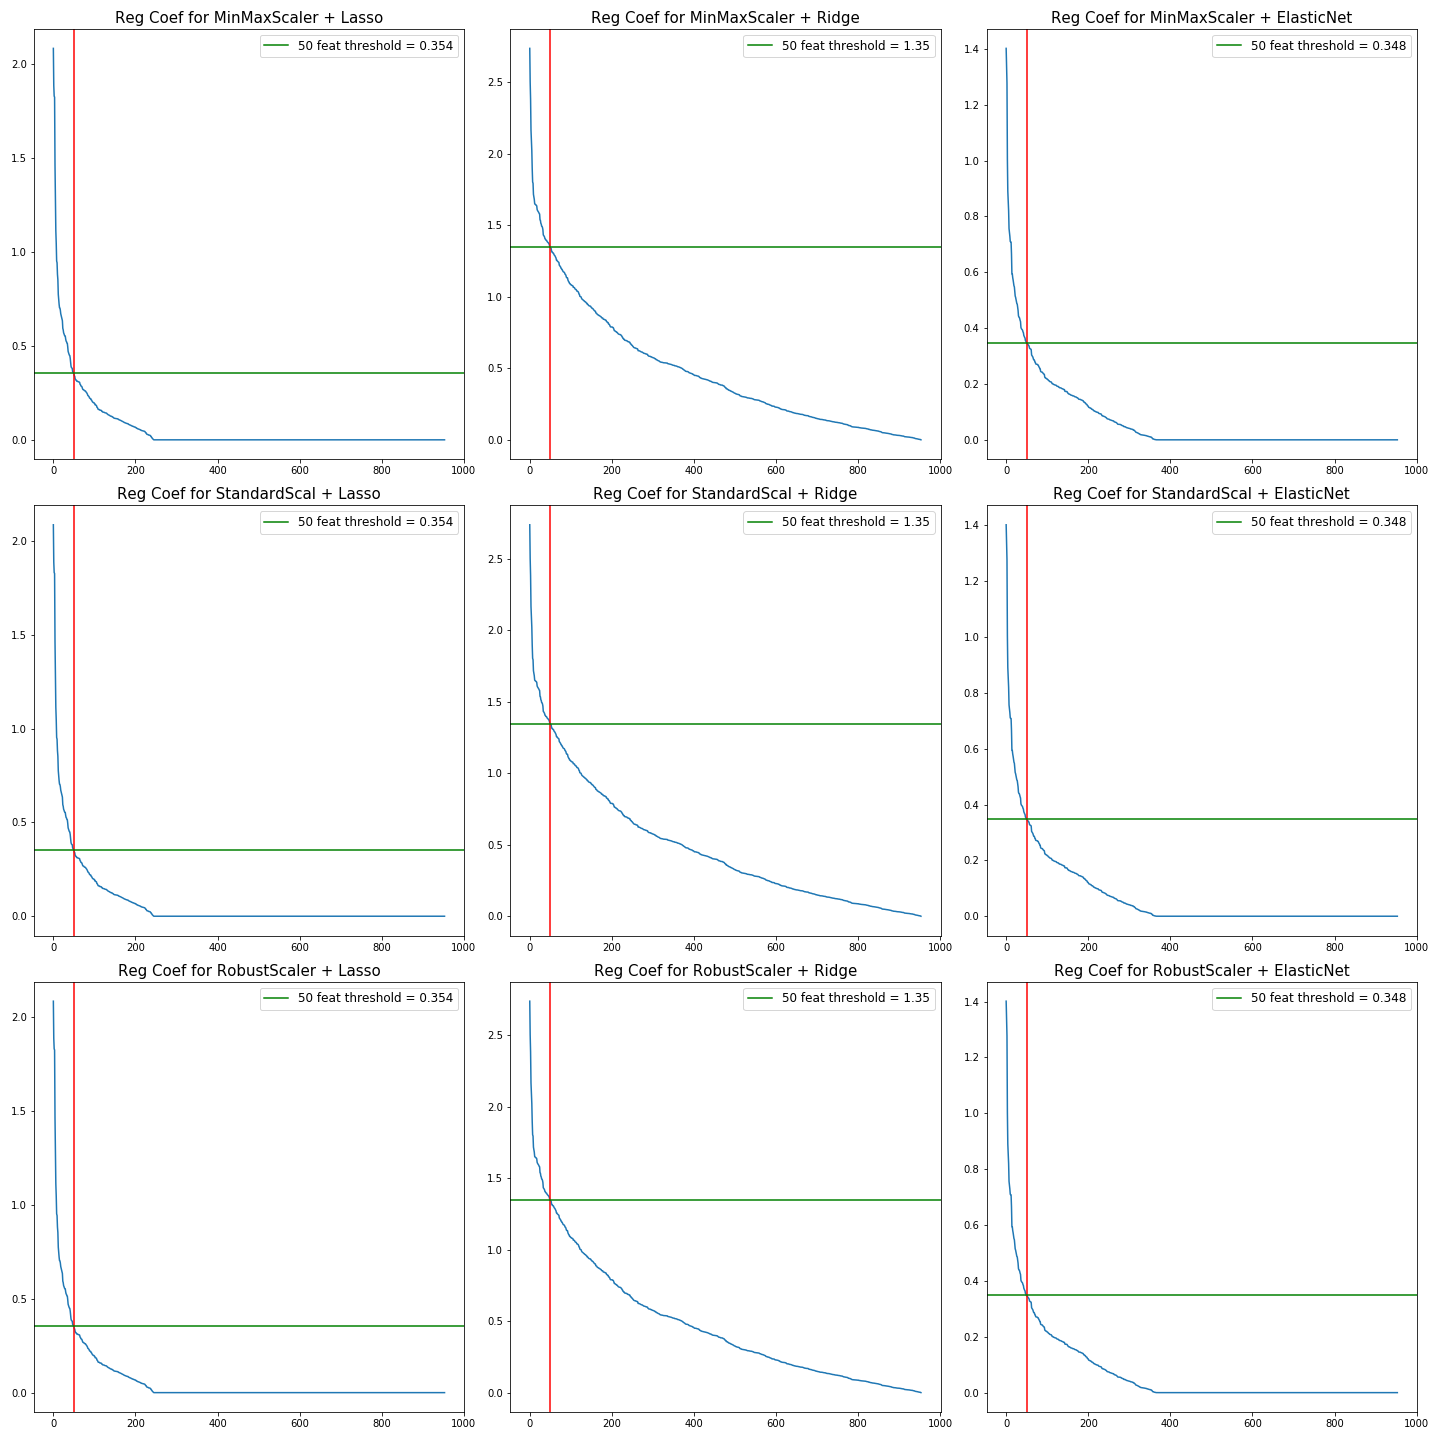
\includegraphics[width=0.9\linewidth]{NineCoefPlot.png}
  \caption{\small{The nine plots that shows the general trend for each one of the scaler + regression combinations. It can be seen that they behave quite the same way. The threshold value does not change at all varying the scaler method, but it depends clearly on the regression method. The vertical red line identify the 50 highest ranked features, while the green horizontal line highlight the threshold value necessary to filter only those features.}}
  \label{fig:NineCoefPlot}
  \end{center}
\end{figure}

What I have actually done to select the features was to implement a custom filter for a set of values using the available packages in the library \texttt{scikitlearn}. In this way I was able to perform the succeeding analysis only on the desired set of features.

\subsection*{Most Influential Features}
The search of the most important features required a ranking system, in order to highlight which ones received generally the highest coefficients among the different regressions. The method I devised it's not based on the effective values but it looks at the presence in top 50, top 25 and top 10 in the nine sets of ordered absolute values of the coefficients. I report below all the 21 features that appear at least once in the top 10 of anyone of the sets of coefficients:

\begin{multicols}{2}
  \begin{verbatim}
    Left.Thalamus.Proper
    Left.Putamen
    Left.Cerebellum.Cortex
    X3rd.Ventricle
    rh.fimbria
    lh_G_front_sup_thickness
    Brain.Stem
    Right.Amygdala
    BrainSegVol.to.eTIV
    Right.Lateral.Ventricle
    lh_superiorfrontal_thickness
    lh_WhiteSurfArea_area
    Right.Cerebellum.White.Matter
    rh_S_postcentral_thickness
    lh.CA4
    lh_G.S_frontomargin_area
    lh_insula_thickness
    rh_supramarginal_thickness
    lh_G_pariet_inf.Angular_volume
    rh_postcentral_thickness
    lh_Pole_occipital_thickness
\end{verbatim}
\end{multicols}

A more exhaustive list of all the 101 features that appear at least once in the top 50 of any of the sets is reported in the appendix.

\subsection*{Regression}
The regression analysis was carried out using a \texttt{GaussianProcessRegressor} onto different reduced set of features using different threshold values on each of the nine arrays. Eventually, a single vector regressor (\texttt{SVR}) has been used on the set of features that gave the best result in the previous passage.

After any dimensionality reduction one expects a drop in the predictive power of the model, and this was the case. The more I filtered the features, selecting only the most influential, the more the $R^{2}$ score dropped. It was necessary to think up a way to find the best compromise between the $R^{2}$ score and the number of features. Thus, I looked for the ratio between these two quantities, in order to select the number at which that value would be the greatest. What I found, as it could be seen in figure \ref{fig:Score_Features_Ratio}, was that also this ratio was dropping as the number of feature was decreasing. Then I chose to use the 50 features with the highest coefficient for the following fine tuning of the parameters. The gaussian process regression in fact do not work well with a too high number of dimensions and 50 was chosen as maximum value.


\begin{figure}[ht!]
  \begin{center}
  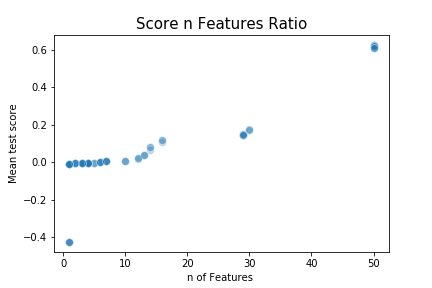
\includegraphics[width=0.7\linewidth]{Score_Features_Ratio.png}
  \caption{\small{In This figure all the value of the ratio between the mean test score and the number of features of that test set are shown. The mean test scores were given by the \texttt{GridScearchCV}. }}
  \label{fig:Score_Features_Ratio}
  \end{center}
\end{figure}


 I used the \texttt{GridScearchCV} item from the \texttt{scikitlearn} library to run the complete pipeline described and find out which would be the highest score combination.

 [Should I report the complete code? pipeline and parameter grid?].

While the gaussian process worked well (scores around 0.68) the best result around $0.72$ was given by a single vector regressor. This result, after a further fine tuning of the parameters, has become $R^{2} = ??$ [The fine tuning in running]. Below it is reported the exact set of parameters used to find this results:

\texttt{[Set of parameter of the best estimator]}


\subsection*{Prediction}
As last step in this data analysis I've used the best \texttt{SVR} regressor to make prediction of age on the test dataset.
Precisely I scaled and filtered according to the most performing combination that was the \texttt{MinMaxScaler} + \texttt{RidgeCV} combination [I'm not sure yet that it is really this one] the test dataset, then used the best \texttt{SVR} regressor previously fitted on the training dataset as a predictor. What I obtained was a set of predicted ages to be put in relation with the target values of the test data set.
I've decided to use a gaussian process to fit those two set of values, because that method is able to provide a good representation of the confidence interval of the prediction over all the range of age. In the figure \ref{fig:SVR_fit} in provided the plot of these two sets of values.

\begin{figure}[H]
  \begin{center}
  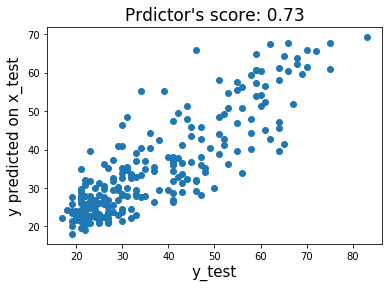
\includegraphics[width=0.5\linewidth]{After_train_SVR.png}
  \caption{\small{Here is reported the scatter plot of the predicted ages versus the target values.[This is still the image without the gaussian process fitting, because I'm still having problems on working it out.]}}
  \label{fig:SVR_fit}
  \end{center}
\end{figure}

As we can see the prediction on the reduced field of features gives a good prediction score, around 0.73 that is quite similar to the score of the fitting on the complete dataset.

\dots


\subsection*{Appendix - Top 50 Features}
This is the list of all the 101 features that appear at least once in the top 50 of any set of coefficients for the nine combinations. The names highlighted in red are the features previously reported as the ones that appear in the top 10.

\begin{multicols}{2}
  \color{red}
  \begin{verbatim}
    Left.Thalamus.Proper
    Left.Putamen
    Left.Cerebellum.Cortex
    X3rd.Ventricle
    rh.fimbria
    lh_G_front_sup_thickness
    Brain.Stem
    Right.Amygdala
    BrainSegVol.to.eTIV
    Right.Lateral.Ventricle
    lh_superiorfrontal_thickness
    lh_WhiteSurfArea_area
    Right.Cerebellum.White.Matter
    rh_S_postcentral_thickness
    lh.CA4
    lh_G.S_frontomargin_area
    lh_insula_thickness
    rh_supramarginal_thickness
    lh_G_pariet_inf.Angular_volume
    rh_postcentral_thickness
    lh_Pole_occipital_thickness
\end{verbatim}
\color{black}
\begin{verbatim}
    lh_rostralmiddlefrontal_thicknessstd
    lh_S_precentral.sup.part_thickness
    rh_G_front_sup_thickness
    X4th.Ventricle
    Right.VentralDC
    lh_S_circular_insula_inf_thicknessstd
    lh_S_circular_insula_sup_thicknessstd
    rh_S_subparietal_area
    lh_posteriorcingulate_area
    lh_G_precuneus_thickness
    lh_supramarginal_thicknessstd
    Left.Caudate
    lh_G_precentral_thicknessstd
    lh_G_temporal_inf_thicknessstd
    rh_G_temp_sup.Lateral_thickness
    lh_lingual_thicknessstd
    lh_G_insular_short_thickness
    rh_fusiform_thickness
    MaskVol.to.eTIV
    rh_superiorfrontal_area
    rh_precentral_area
    lh_lateraloccipital_volume
    rh_inferiortemporal_area
    lh_S_interm_prim.Jensen_area
    lh_S_circular_insula_sup_area
    rh_G.S_subcentral_volume
    lh_inferiorparietal_thickness
    lh_S_circular_insula_sup_volume
    lh_S_interm_prim.Jensen_volume
    lh_S_parieto_occipital_volume
    lh_S_temporal_sup_volume
    rh_S_occipital_ant_thickness
    rh_S_precentral.sup.part_thickness
    lh_parsopercularis_thicknessstd
    lh_S_circular_insula_sup_thickness
    lh_S_oc_middle.Lunatus_thickness
    lh_S_orbital.H_Shaped_thickness
    lh_S_temporal_inf_thickness
    Left.VentralDC
    rh_S_circular_insula_inf_thicknessstd
    WM.hypointensities
    SubCortGrayVol
    lh_S_orbital.H_Shaped_thicknessstd
    rh_parsopercularis_thicknessstd
    lh_G_postcentral_area
    lh_S_central_area
    lh_S_circular_insula_inf_area
    rh_S_circular_insula_inf_volume
    lh_parstriangularis_thickness
    rh_G_postcentral_thickness
    rh_G_temporal_inf_thickness
    lh_S_circular_insula_inf_thickness
    lh_G_temporal_middle_thickness
    rh_transversetemporal_thickness
    rh_parstriangularis_thickness
    Left.Lateral.Ventricle
    Right.Thalamus.Proper
    lh.fimbria
    rh_precuneus_area
    rh_supramarginal_area
    rh_G.S_frontomargin_area
    rh_S_pericallosal_area
    rh_Pole_occipital_area
    lh_isthmuscingulate_area
    lh_lingual_area
    lh_medialorbitofrontal_area
    lh_superiorfrontal_area
    lh_S_parieto_occipital_area
    lh_S_postcentral_area
    lh_Lat_Fis.ant.Horizont_area
    rh_G_parietal_sup_volume
    lh_superiorfrontal_volume
    lh_supramarginal_volume
    lh_insula_volume
    lh_G.S_frontomargin_volume
    lh_G_cuneus_volume
    rh_inferiortemporal_volume
    rh_superiortemporal_volume
  \end{verbatim}
\end{multicols}



\end{document}
